\documentclass[border=5pt]{standalone}
\usepackage{tikz}
\usepackage{xcolor}
\usetikzlibrary{arrows.meta,shapes,positioning,patterns,decorations.pathmorphing,calc}

\definecolor{shaft}{RGB}{90,90,90}
\definecolor{backiron}{RGB}{60,90,110}
\definecolor{magnetN}{RGB}{180,50,50}
\definecolor{magnetS}{RGB}{50,50,180}
\definecolor{statorteeth}{RGB}{139,90,60}
\definecolor{phaseA}{RGB}{255,150,50}
\definecolor{phaseB}{RGB}{255,200,50}
\definecolor{phaseC}{RGB}{200,150,100}

\begin{document}
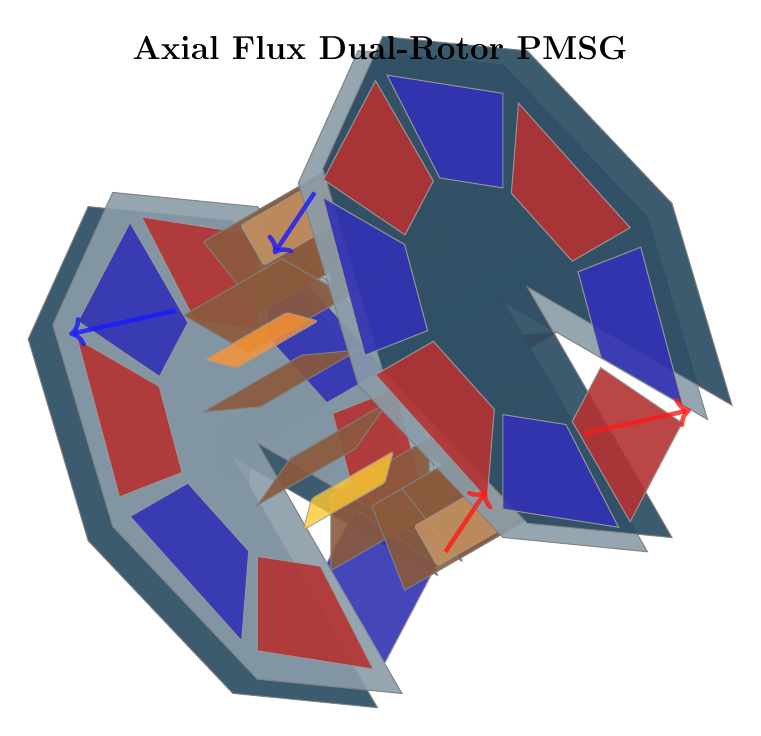
\begin{tikzpicture}[scale=1.2,
    x={(0.866cm,-0.5cm)}, y={(0cm,1cm)}, z={(0.866cm,0.5cm)}]

  % Central Shaft
  \draw[fill=shaft!120, opacity=0.95, draw=black!60] (0,0,-2) -- (0,0,2) -- (0,0.4,2) -- (0,0.4,-2) -- cycle;
  \draw[fill=shaft!70, opacity=0.95, draw=black!60] (0,0,2) -- (0.4,0,2) -- (0.4,0.4,2) -- (0,0.4,2) -- cycle;
  \draw[fill=shaft!50, opacity=0.95, draw=black!60] (0,0,-2) -- (0.4,0,-2) -- (0.4,0.4,-2) -- (0,0.4,-2) -- cycle;

  % Left Rotor Back Iron
  \draw[fill=backiron!110, opacity=0.90, draw=black!50] (0,0,-1.8)
    \foreach \ang in {0,45,...,315} { -- ({2.5*cos(\ang)}, {2.5*sin(\ang)}, -1.8) } -- cycle;
  \draw[fill=backiron!60, opacity=0.90, draw=black!50] (0,0,-1.5)
    \foreach \ang in {0,45,...,315} { -- ({2.5*cos(\ang)}, {2.5*sin(\ang)}, -1.5) } -- cycle;

  % Left Rotor Magnets
  \foreach \ang/\col in {0/magnetN, 45/magnetS, 90/magnetN, 135/magnetS,
                         180/magnetN, 225/magnetS, 270/magnetN, 315/magnetS} {
    \draw[fill=\col, opacity=0.90, draw=black!40]
      ({1.2*cos(\ang)}, {1.2*sin(\ang)}, -1.5) -- ({2.2*cos(\ang)}, {2.2*sin(\ang)}, -1.5) --
      ({2.2*cos(\ang+40)}, {2.2*sin(\ang+40)}, -1.5) -- ({1.2*cos(\ang+40)}, {1.2*sin(\ang+40)}, -1.5) -- cycle;
  }

  % Stator Teeth
  \foreach \ang in {0,30,...,330} {
    \draw[fill=statorteeth, opacity=0.90, draw=black!50]
      ({1.0*cos(\ang)}, {1.0*sin(\ang)}, -0.6) -- ({1.8*cos(\ang)}, {1.8*sin(\ang)}, -0.6) --
      ({1.8*cos(\ang)}, {1.8*sin(\ang)}, 0.6) -- ({1.0*cos(\ang)}, {1.0*sin(\ang)}, 0.6) -- cycle;
  }

  % Three-Phase Windings
  \foreach \ang/\col in {15/phaseA, 75/phaseB, 135/phaseC, 195/phaseA, 255/phaseB, 315/phaseC} {
    \draw[fill=\col, opacity=0.80, rounded corners=1pt, draw=black!40]
      ({1.3*cos(\ang)}, {1.3*sin(\ang)}, -0.5) -- ({1.7*cos(\ang)}, {1.7*sin(\ang)}, -0.5) --
      ({1.7*cos(\ang)}, {1.7*sin(\ang)}, 0.5) -- ({1.3*cos(\ang)}, {1.3*sin(\ang)}, 0.5) -- cycle;
  }

  % Right Rotor Back Iron
  \draw[fill=backiron!60, opacity=0.90, draw=black!50] (0,0,1.5)
    \foreach \ang in {0,45,...,315} { -- ({2.5*cos(\ang)}, {2.5*sin(\ang)}, 1.5) } -- cycle;
  \draw[fill=backiron!110, opacity=0.90, draw=black!50] (0,0,1.8)
    \foreach \ang in {0,45,...,315} { -- ({2.5*cos(\ang)}, {2.5*sin(\ang)}, 1.8) } -- cycle;

  % Right Rotor Magnets
  \foreach \ang/\col in {0/magnetS, 45/magnetN, 90/magnetS, 135/magnetN,
                         180/magnetS, 225/magnetN, 270/magnetS, 315/magnetN} {
    \draw[fill=\col, opacity=0.90, draw=black!40]
      ({1.2*cos(\ang)}, {1.2*sin(\ang)}, 1.5) -- ({2.2*cos(\ang)}, {2.2*sin(\ang)}, 1.5) --
      ({2.2*cos(\ang+40)}, {2.2*sin(\ang+40)}, 1.5) -- ({1.2*cos(\ang+40)}, {1.2*sin(\ang+40)}, 1.5) -- cycle;
  }

  % Flux arrows
  \draw[->, ultra thick, red!90, opacity=0.8] (2.3,0,-1.5) -- (1.9,0,-0.6);
  \draw[->, ultra thick, red!90, opacity=0.8] (1.9,0,0.6) -- (2.3,0,1.5);
  \draw[->, ultra thick, blue!90, opacity=0.8] (-2.3,0,1.5) -- (-1.9,0,0.6);
  \draw[->, ultra thick, blue!90, opacity=0.8] (-1.9,0,-0.6) -- (-2.3,0,-1.5);

  % Title label
  \node[font=\large\bfseries, anchor=south] at (0,3.2,0) {Axial Flux Dual-Rotor PMSG};

\end{tikzpicture}
\end{document}
